\documentclass{beamer}
\mode<presentation> {}
\usepackage{graphicx, booktabs, float, subfig}

\title[Subtitle]{Image Classification Using Convolutional Neural Nets}
\author{C. Aden, C. Qin, and N. Ulle}
\institute[]{University of California, Davis \medskip}
\date{}

\begin{document}
\begin{frame}
\titlepage
\end{frame}

\begin{frame}
\frametitle{Introduction to CNN}
Convolutional Neural Networks (CNNs) are variants of \emph{multilayer perceptrons}, inspired by the cell arrangement within the visual cortex. \vspace{0.2cm}\\
\textbf{How it roughly works}: Extracting different types of \emph{local features} from the input image. 
\begin{figure}
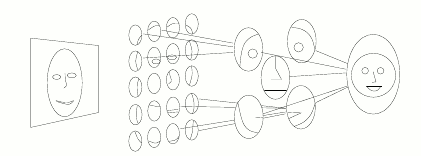
\includegraphics[width=0.5\linewidth]{face.jpeg}
\end{figure}
\textbf{Key feature}: Invariance to geometric transformations (\emph{shift, scale and distortion}) of the input. Allows us to detect features regardless of position in a picture.
\end{frame}

\begin{frame}
\frametitle{Elements of CNN} 
\begin{itemize} 
\item A \textbf{convolutional layer} has the following two components:
\begin{itemize}
\item \emph{Local receptive fields} enable the network to extract elementary visual features, e.g., oriented edges, end-points, and corners.
\begin{figure}
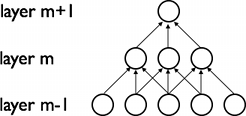
\includegraphics[width=0.3\linewidth]{sparse.jpeg}
\end{figure}
\item \emph{Shared weights} allows for features to be detected regardless of their position in the visual field.
\end{itemize}
\begin{figure}
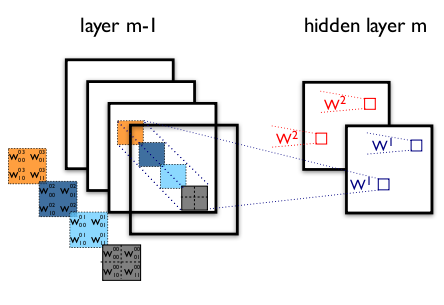
\includegraphics[width=0.35\linewidth]{weight.jpeg}
\end{figure}
\item \textbf{Sub-sampling layer} reduces the number of free parameters (spatial resolution) and provides translation invariance.
\end{itemize}
\end{frame}

\begin{frame}
\frametitle{Architecture of CNN} 
A CNN consists of \emph{alternating} convolution and sub-sampling layers. \vspace{0.3cm}
\begin{figure}
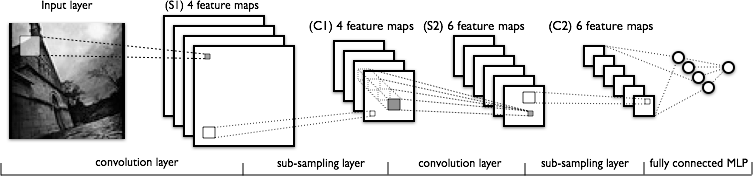
\includegraphics[width=0.9\linewidth]{CNN.jpeg}
\end{figure}
\vspace{0.4cm}
The invariance to translation and distortion of the input is achieved by a progressive increase of the number of feature maps coupled with a progressive reduction of spatial resolution. 
\end{frame}


\begin{frame}
\frametitle{The OverFeat Program} 
\begin{itemize}
\item Convolutional Neural Network, pre-trained on the ImageNet image hierarchy database (14.2 million images).
\item Written in C++, can be compiled to work on the GPU, or with a tuned BLAS.
\item Extracts features from images, to be used in classification.
\end{itemize}
\end{frame}

\begin{frame}
\frametitle{Our Approach} 
\begin{itemize}
\item Run OverFeat on the training images ($20,000$) to generate features.
\item Max-pool over the feature layers to reduce the space ($1 \times 4096$ for each image)
\item Use the $20,000 \times 4096$ features matrix, along with labels to train a support vector machine.
\item Run OverFeat on the $5,000$ testing images.
\item Using the trained SVM classifier, assign 'cat' or 'dog' to each image and store the probability of that decision.
\end{itemize}
\end{frame}

\begin{frame}
\frametitle{Results}
Results through Cross-Validation on Training Data (5\% held-out):
\begin{itemize}
\item Classifying based on pixel values with Radial Basis Function SVM: 57\% (recall that guessing is about 50\%).
\item Classifying ImageNet labels from OverFeat: 88.7\%.
\item ImageNet feature layer with linear-kernel SVM: 95\%
\item ImageNet feature layer with cubic polynomial-based kernel SVM: 96\%
\item ImageNet feature layer with Radial Basis Function-based kernel SVM: 98\%
\end{itemize}
\end{frame}

\begin{frame}
\frametitle{Difficulties}
\begin{itemize}
\item Non-dog/cat images (ex: picture of a rose, image of text, hand-drawn cat, 0KB image)
\item Cats and dogs in strange poses
\item Very small images (smaller than $100 \times 100$). They were enlarged in Python to allow the algorithm work, but classification rate suffered.
\end{itemize}
\end{frame}
\end{document} 